%─────────────────────────────────────────────────────────────────────────────
% main.tex
% Wissenschaftliche Projektarbeit (ca. 30 Seiten) mit modularen Kapiteln
%─────────────────────────────────────────────────────────────────────────────
\documentclass[
    paper=a4,                % A4-Papier
    fontsize=11pt,           % 11pt Schriftgröße
    headings=normal,         % Normale Kapitälchen-Überschriften
    parskip=half,            % Halbzeiliger Abstand zwischen Absätzen
    listof=totoc,            % Abbildungsverzeichnis ins Inhaltsverzeichnis
    bibliography=totoc,      % Literaturverzeichnis ins Inhaltsverzeichnis
    toc=bibliography,        % Inhaltsverzeichnis mit Bibliographie-Nummer
    chapterprefix=false      % „Kapitel“-Präfix weglassen, falls gewünscht
]{scrreprt}

% ─────────────────────────────────────────────────────────────────────────────
% Paket‐Ladebefehle und Grundeinstellungen
% ─────────────────────────────────────────────────────────────────────────────
\usepackage[T1]{fontenc}              % T1 Kodierung (Trennung von Umlauten)
\usepackage[utf8]{inputenc}           % UTF-8 Eingabekodierung
\usepackage[ngerman]{babel}           % Deutsche Dokumentensprache
\usepackage{csquotes}                 % Korrekte Anführungszeichen, benötigt von biblatex
\usepackage{microtype}                % Verbesserte typografische Feineinstellungen
\usepackage[hyphens]{url}


% Abstand & Layout
\usepackage{setspace}                 % Zeilenabstand: \onehalfspacing, \doublespacing
\onehalfspacing                       % 1,5-zeiliger Abstand (De-facto Standard)
\usepackage{geometry}                 
\geometry{
  a4paper,
  left=30mm,
  right=25mm,
  top=25mm,
  bottom=25mm
}

% Kopf-/Fußzeilen
\usepackage[automark]{scrlayer-scrpage}
\clearpairofpagestyles
\ihead{\headmark}                     % Kapitelüberschrift in den Kopf
\ofoot{\pagemark}                     % Seitennummer im Fuß
\setkomafont{pageheadfoot}{\small}    % kleine Schrift in Kopf/Fuß

% Grafiken und Tabellen
\usepackage{graphicx}                 
\usepackage{caption}                  
\usepackage{subcaption}               % Unterabbildungen
\usepackage{booktabs}                 % Professionelle Tabellenlinien
\usepackage{tabularx}                 % Erweiterte Tabellenspalten
\usepackage{longtable}                % Tabellen, die sich über Seiten erstrecken

% Mathematik
\usepackage{amsmath,amssymb,amsthm}    % Mathe‐Umgebungen und Symbole

% Farben, Quellcode, Hyperlinks
\usepackage{xcolor}                   
\usepackage{listings}                 % Quellcode-Auszeichnung
\usepackage{hyperref}                 
\hypersetup{
    colorlinks=true,
    linkcolor=blue,
    citecolor=blue,
    urlcolor=blue
}
\usepackage{cleveref}                 % Intelligente Verweise: \cref, \Cref

% Bibliographie (BibLaTeX)
\usepackage[
    backend=biber,                    % biber als Backend
    style=alphabetic,                 % z.B. alphabetischer Stil (kann angepasst werden)
    citestyle=authoryear,             % Zitierstil: (Autor Jahr)
    sorting=nyt,                      % Sortierung: Name, Jahr, Titel
]{biblatex}
\addbibresource{literature.bib}       % Deine BibTeX-Datei

% Eigene Makros, Definitionen (falls benötigt)
\newcommand{\HRule}{\rule{\linewidth}{0.5mm}}   % Horizontaler Strich
% … hier kannst du weitere Makros definieren

% ─────────────────────────────────────────────────────────────────────────────
% Beginn des Dokuments
% ─────────────────────────────────────────────────────────────────────────────
\begin{document}

% Titelseite
%─────────────────────────────────────────────────────────────────────────────
% Titelseite deiner Projektarbeit
%─────────────────────────────────────────────────────────────────────────────
\thispagestyle{empty}
\begin{titlepage}
    \begin{center}
        \vspace*{2cm}
        {\Huge\textbf{Erkennung von Deepfakes\\ mittels Convolutional Neural Networks}}\\
        \vspace{1cm}
        {\Large Projektarbeit im Studiengang Informatik}\\
        \vspace{2cm}

        {\Large \textbf{Vorname Nachname}}\\
        \vspace{0.5cm}
        Matrikelnummer: 1234567\\
        \vspace{1cm}

       % \includegraphics[width=0.4\textwidth]{figures/universitaet-logo.png}\\   % ggf. Logo einfügen
        \vspace{1cm}

        {\large Abgabedatum: 05.\ Juni 2025}\\
        \vfill

        Betreuer: Prof. Dr. Max Mustermann\\
        Zweitkoordinator: Dr. Erika Beispiel
    \end{center}
\end{titlepage}


% Abstract (Zusammenfassung)
%─────────────────────────────────────────────────────────────────────────────
% Kurze Zusammenfassung (Abstract) auf Deutsch, 150–250 Wörter
%─────────────────────────────────────────────────────────────────────────────
\chapter*{Abstract}
\addcontentsline{toc}{chapter}{Abstract}

Im Rahmen dieser Projektarbeit wird untersucht, wie Convolutional Neural Networks (CNNs) eingesetzt werden können, um Deepfake-Bilder von echten Aufnahmen zu unterscheiden. Dazu werden verschiedene Datensätze (u. a. Kaggle–Deepfake‐Datensätze) zusammengeführt, vorverarbeitet und als Trainings- und Validierungssets aufbereitet. Als Basis dient ein vortrainiertes ResNet50‐Netzwerk, das durch Transfer Learning auf die Erkennung von Deepfakes adaptiert wird. Der Trainingsprozess umfasst sowohl das Einfrieren der Basislayer als auch ein anschließendes Fine-Tuning. Die Ergebnisse werden anhand von Kennzahlen wie Accuracy, Precision, Recall, F1-Score und AUC evaluiert. Abschließend werden Limitationen und mögliche Verbesserungsstrategien diskutiert. 


% Inhaltsverzeichnis
\clearpage
\tableofcontents
\clearpage

% ─────────────────────────────────────────────────────────────────────────────
% 1. Einleitung
% ─────────────────────────────────────────────────────────────────────────────
%─────────────────────────────────────────────────────────────────────────────
% Kapitel 1: Einleitung
%─────────────────────────────────────────────────────────────────────────────
\chapter{Einleitung}
\label{chap:einleitung}

Deepfakes sind synthetisch erzeugte Medien, bei denen das Gesicht einer Person realistisch in Video- oder Bildmaterial eingefügt wird. Mit wachsender Rechenleistung und verbesserten Algorithmen lassen sich derartige Fälschungen immer schwieriger mit bloßem Auge erkennen. Die damit einhergehenden Risiken reichen von politischer Manipulation bis hin zum Identitätsdiebstahl. Ziel dieser Arbeit ist es, auf Basis moderner Deep-Learning‐Techniken automatische Verfahren zur Erkennung von Deepfakes zu entwickeln und zu evaluieren.

In den letzten Jahren wurden zahlreiche Methoden vorgestellt, die tiefe neuronale Netze nutzen, um Artefakte in Deepfake-Bildern zu detektieren (vgl. \cite{agarwal2020detecting}, \cite{rossler2019faceforensics++}). Viele Arbeiten beschränken sich auf bestimmte Arten von Deepfake‐Algorithmen (z. B. GAN‐basiert), während andere einen breiteren Ansatz wählen, der auf Merkmale wie unnatürliche Augenreflexion, fehlende Gesichtsmerkmale oder Inkonsistenzen in den Spatial-Frequenzen abzielt. 

In Kapitel \ref{chap:datensaetze} werden die verwendeten Datensätze genauer beschrieben. Kapitel \ref{chap:methodik} stellt die grundlegende Methodik vor, gefolgt von technischen Details zur Implementierung in Kapitel \ref{chap:implementierung}. Die experimentelle Evaluation und die erzielten Ergebnisse sind in Kapitel \ref{chap:evaluation} zusammengefasst. Abschließend erfolgt in Kapitel \ref{chap:diskussion} eine kritische Reflexion der gefundenen Resultate, bevor in Kapitel \ref{chap:fazit} ein Fazit gezogen wird.


% ─────────────────────────────────────────────────────────────────────────────
% 2. Datensätze
% ─────────────────────────────────────────────────────────────────────────────
\input{chapters/05_Datensätze.tex}

% ─────────────────────────────────────────────────────────────────────────────
% 3. Methodik
% ─────────────────────────────────────────────────────────────────────────────
%─────────────────────────────────────────────────────────────────────────────
% Kapitel 3: Methodik
%─────────────────────────────────────────────────────────────────────────────
\chapter{Methodik}
\label{chap:methodik}

Die entwickelte Methodik ist in zwei exemplarische Implementierungen gegliedert, die unter den Bezeichnungen „Versuch 1“ und „Versuch 2“ ausführlich beschrieben werden. Beide verfolgen das Ziel, ein robustes Bildklassifikationssystem zur Unterscheidung zwischen echten und manipulierten Gesichtern („Deepfakes“) zu entwickeln und zu evaluieren. Trotz unterschiedlicher technischer Schwerpunkte – einmal der Einsatz eines ResNet-50-Backbones, einmal die Verwendung des schlankeren MobileNetV2-Netzes mit einer eigenen Datenpipeline – folgen beide Implementierungen demselben strukturellen Rahmen, der im Folgenden dargestellt wird.

Zu Beginn jeder Variante steht die automatische Erkennung der Rechenressourcen. Durch Abfrage verfügbarer GPU-Devices wird sichergestellt, dass die Trainingsschritte mit maximaler Effizienz auf spezialisierten Tensor-Cores ausgeführt werden können; fehlt eine GPU, fällt das System automatisch auf CPU-Berechnung zurück. Unmittelbar danach aktiviert die Mixed-Precision–Policy (16-Bit vs. 32-Bit) ein flexibles Training, das sowohl Geschwindigkeit als auch Speicherauslastung optimiert, ohne nennenswerte Einbußen bei der numerischen Stabilität in Kauf zu nehmen.

Ein zentrales Element beider Pipelines ist die sorgfältige Datenvorverarbeitung. Rohbilder werden über eine auf Haar-Cascades basierende Gesichtsdetektion in Region-of-Interest–Ausschnitte transformiert. Diese klassische Computer-Vision-Methode gewährleistet, dass ausschließlich relevante Bildbereiche – also tatsächliche Gesichter – dem tiefen neuronalen Netz als Input zugeführt werden. Durch anschließendes Resizing und standardisiertes Preprocessing (Normierung auf die von den vortrainierten Keras-Modellen erwarteten Wertebereiche) wird eine konsistente Eingaberepräsentation geschaffen, die das Fine-Tuning der Convolutional-Backbones optimal unterstützt.

Die Daten werden in beiden Verfahren batch-weise nachgeladen; im ersten Ansatz geschieht dies mit Hilfe von Keras’ internem `ImageDataGenerator`, im zweiten durch eine speziell implementierte `Sequence`-Klasse, die neben dem Laden und Preprocessing eine automatische Filterung und Beschneidung von Bildern realisiert. Beide Varianten gewährleisten, dass der Arbeitsspeicher nicht durch komplette Datensätze überlastet wird, sondern nur jeweils die für den aktuellen Trainingsschritt notwendigen Batches vorgehalten werden.

Kernstück jeder Pipeline ist das Transfer-Learning: Ein vortrainiertes Convolutional Neural Network (ResNet-50 oder MobileNetV2) dient als Feature-Extraktor, dessen Gewichte zunächst aus dem ImageNet-Training übernommen und im weiteren Verlauf feingetunt werden. In beiden Fällen wird der „Top“-Klassifikator entfernt und durch eine Kombination aus GlobalAveragePooling, einem dichten Hidden-Layer mit ReLU-Aktivierung und L2-Regularisierung sowie einer abschließenden Sigmoid-Ausgabe ersetzt. Dropout-Schichten mit hoher Rate (50–60 %) reduzieren Overfitting weiter, während der Adam-Optimierer zusammen mit binärer Kreuzentropie als Verlustfunktion eine effiziente Parameteranpassung sicherstellt.

Um die Trainingsdynamik adaptiv zu steuern, kommen in beiden Implementierungen Callback-Mechanismen zum Einsatz: Checkpoints speichern das beste Modell anhand der Validierungsgenauigkeit, Learning-Rate-Scheduler reduzieren die Lernrate bei stagnierendem Verlust, und TensorBoard-Logs dokumentieren Metriken und Gewichthistogramme. Auf diese Weise kann das Training komfortabel überwacht und analysiert werden.

Die abschließende Evaluierung erfolgt auf einem separaten Testdatensatz. Neben der üblichen Ausgabe von Loss- und Accuracy-Werten werden detaillierte Klassifikationsreports und Konfusionsmatrizen erzeugt. Im zweiten Versuch werden zudem falsch klassifizierte Bilder automatisch extrahiert und gespeichert, um eine gezielte Fehlermusteranalyse zu ermöglichen.

Insgesamt bildet diese Methodik einen modularen, erweiterbaren Rahmen: Von der Hardware-Erkennung und Mixed-Precision über datengetriebene Vorverarbeitung und moderne Transfer-Learning-Techniken bis hin zu adaptivem Trainings-Monitoring und umfassender Evaluierung. Die beiden Versuche illustrieren unterschiedliche Wege zu demselben Ziel und bieten eine solide Grundlage für weiterführende Optimierungen, etwa durch Datenaugmentation, Ensemble-Methoden oder alternative Backbone-Architekturen.

\section{Versuch 1}

Der erste Traningsversuch verfolgt das Ziel, auf Basis eines vortrainierten ResNet-50-Netzwerks ein binäres Klassifikationsmodell für Bilddaten zu erstellen, zu trainieren, zu validieren und letztlich zu testen. Dabei wird ein durchgängiger Workflow realisiert, der von der Hardware-Erkennung und Konfigurationsanpassung über die Datenaufbereitung und Modelldefinition bis hin zu Trainings-Monitoring, automatischer Lernratenanpassung und abschließender Leistungsbeurteilung reicht.

Zu Beginn erfolgt eine Abfrage der verfügbaren Hardware: Mittels \nolinkurl{tf.config.list_physical_devices('GPU')} wird ermittelt, ob eine oder mehrere NVIDIA-GPUs im System zur Verfügung stehen. GPUs sind für das Training tiefer neuronaler Netze aufgrund ihrer hohen Parallelrechenleistung nahezu unerlässlich, da sie große Matrizenoperationen wesentlich effizienter als CPUs abarbeiten können. Findet der Code GPU(s), so wird ihre Existenz dem Anwender angezeigt; andernfalls fällt der Workflow auf CPU-Berechnung zurück. Diese dynamische Hardware-Erkennung erhöht die Portabilität des Skripts und stellt sicher, dass es sowohl auf Entwickler-Workstations mit GPU als auch in reinen CPU-Umgebungen lauffähig ist.

Unmittelbar danach wird Mixed-Precision-Training aktiviert. Hierzu importiert das Skript aus \texttt{tensorflow.keras.mixed\_precision} die Klasse \texttt{Policy} mit dem Argument \texttt{'mixed\_float16'} und setzt diese als globale Policy. Mixed Precision kombiniert 16-Bit-Gleitkomma-Darstellung für die meisten Netzwerksoperationen mit 32-Bit-Darstellung für solche Teile, in denen dies numerisch kritisch ist (z.\,B. Skalierungsoperationen für den Gradienten). Durch die halbierte Speicherbelegung und den effizienteren Datendurchsatz moderner GPUs kann so eine erhebliche Beschleunigung des Trainings erreicht werden, ohne dabei signifikante Genauigkeitsverluste hinzunehmen. Dies ist insbesondere bei großen Netztiefen wie ResNet-50 von Vorteil.

Anschließend werden sämtliche benötigten Bibliotheken importiert: Neben TensorFlow und dem Keras-API zur Modellierung kommt die \texttt{ImageDataGenerator}-Klasse zur dynamischen Datenvorverarbeitung ins Spiel, während \texttt{sklearn.metrics} das Auswerten von Klassifikationszielen durch Berichte und Matrizen ermöglicht. Zusätzlich werden \texttt{os} und \texttt{datetime} für Pfadmanagement und Zeitstempel-Generierung genutzt – essenziell, um etwa Trainingsprotokolle und Modellcheckpoints klar zu strukturieren.

Die Parameter für Bildgröße und Batch-Größe werden festgelegt: \texttt{img\_width} und \texttt{img\_height} betragen jeweils 256 Pixel, womit alle Eingabebilder auf eine einheitliche Quadratform gebracht werden. Die Wahl dieses Formats beruht auf einem Kompromiss zwischen Detailgenauigkeit (größere Auflösung) und Rechenaufwand (kleinere Bilder reduzieren Speicherbedarf und Rechenzeit). Die Batch-Größe von 64 stellt einen gängigen Wert dar, der bei GPUs mit ausreichend Arbeitsspeicher stabile Trainingsverläufe ermöglicht, ohne den Hauptspeicher zu überlasten. Darüber hinaus wird die Anzahl der initialen Epochen (\texttt{initial\_epochs}) auf 50 festgelegt, um dem Modell ausreichend viele Durchläufe über den Datensatz zu gewähren.

Für die Datenaufbereitung kommen je Verzeichnis (Training, Validierung, Test) Instanzen von \texttt{ImageDataGenerator} zum Einsatz, wobei als einzige Transformation die ResNet-Vorverarbeitung (\texttt{preprocess\_input}) zur Normierung auf die für das vortrainierte Modell erwarteten Wertebereiche erfolgt. Dies umfasst das Subtrahieren der ImageNet-Mittelwerte und entsprechende Skalierung. Auf weitergehende Augmentierungen wie Rotationen oder Spiegelungen wird hier verzichtet, kann aber leicht ergänzt werden, um die Robustheit gegen Überanpassung zu erhöhen.

Die Generatoren selbst (\texttt{flow\_from\_directory}) lesen die Bilddateien direkt aus den vorgegebenen Ordnerstrukturen \texttt{Dataset/train}, \texttt{Dataset/validation} und – optional – \texttt{Dataset/test} ein. Durch die Parametrisierung mittels \texttt{target\_size}, \texttt{batch\_size} und \texttt{class\_mode='binary'} werden die Bilder passend formatiert und die zugehörigen binären Labels erwartet. Die Methode stellt sicher, dass die Daten bei jedem Trainingsdurchlauf in Batches fließend nachgeladen werden, ohne den gesamten Datensatz permanent im Arbeitsspeicher halten zu müssen.

Im Kern des Modells steht das vortrainierte ResNet-50, geladen mit Gewichten aus dem ImageNet-Datensatz. Die Verwendung von \texttt{include\_top=False} entfernt die ursprüngliche Klassifikationsschicht, sodass das Netzwerk als reiner Feature-Extraktor dient. Die Eingangsform von \texttt{(256, 256, 3)} entspricht den definierten Bildgrößen. Alle Layer des Basismodells werden dabei auf trainierbar belassen (\texttt{base\_model.trainable = True}), um feingranulare Anpassungen an die neue Aufgabe zu ermöglichen – ein Ansatz, der als Fine-Tuning bekannt ist.

Auf diesen Feature-Extractor schließt sich ein Sequential-Modell-Aufbau an: Zunächst wird mittels \texttt{GlobalAveragePooling2D()} der räumliche Durchschnitt über die Feature-Maps gebildet, wodurch aus einer dreidimensionalen Tensorstruktur ein eindimensionaler Vektor resultiert. Anschließend folgt ein Dense-Layer mit 128 Neuronen und ReLU-Aktivierung, der durch einen L2-Regularisierer (\texttt{l2(0.002)}) kontrolliert wird. Die Regularisierung fügt dem Verlust eine Strafe für hohe Gewichtswerte hinzu, um Overfitting entgegenzuwirken. Um den Regularisierungseffekt zu verstärken, wird ein \texttt{Dropout(0.6)} mit einer Rate von 60 \% eingesetzt: In jedem Trainingsschritt werden zufällig 60 \% der Neuronen dieses Layers inaktiv gesetzt, was Netzwerkeinheiten zur Bildung redundanter Repräsentationen zwingt und so Generalisierung fördert. Abschließend schließt eine Ausgabeschicht mit einem Neuron und Sigmoid-Aktivierung den Aufbau ab, um eine Wahrscheinlichkeitsprognose für die binäre Klassenzugehörigkeit zu erzeugen. Die Ausgabe wird explizit auf den Datentyp \texttt{float32} umgewandelt, um Kompatibilität mit Verlust- und Metrikberechnungen zu garantieren.

Die Kompilierung des Modells erfolgt mit dem Adam-Optimierer, der adaptive Lernraten für jede Netzwerkgewichtung berechnet, sowie dem binären Kreuzentropie-Verlust, der sich für dichotome Klassifikationsaufgaben als Standard etabliert hat. Als Metrik wird die Genauigkeit (\texttt{accuracy}) gewählt, um den Anteil korrekt klassifizierter Beispiele zu überwachen.

Zur Überwachung und Steuerung des Trainings werden drei Callback-Instanzen definiert:
\begin{itemize}
  \item \textbf{ModelCheckpoint} sichert nach jeder Epoche nur dann die Gewichte in \texttt{best\_model\_initial.h5}, wenn sich die Validierungsgenauigkeit verbessert. So kann das Modell mit dem besten Validierungsergebnis später erneut geladen werden.
  \item \textbf{ReduceLROnPlateau} überwacht den Validierungsverlust und senkt bei ausbleibendem Fortschritt (10 Epochen ohne Verbesserung) den Lernratenparameter um den Faktor 0,2, bis zu einem Minimalwert von 1e-7. Das verhindert ein Verharren in Plateaus des Optimierungsprozesses.
  \item \textbf{TensorBoard} protokolliert Metriken, Verluste und – auf Wunsch – Histogramme der Gewichte im Verlauf des Trainings. Die Protokolle werden unter einem Verzeichnis \texttt{logs/fit/<Zeitstempel>} abgelegt, wodurch sie über die TensorBoard-Weboberfläche visualisiert werden können.
\end{itemize}

Das eigentliche Training wird durch \texttt{model.fit()} angestoßen, wobei die Schritte pro Epoche (\texttt{steps\_per\_epoch}) und Validierungsschritte auf ganzzahlige Vielfache der Batchgröße verteilt werden. Die Option \texttt{workers=4} ermöglicht einen parallelen Datengenerator-Betrieb mit vier Arbeitsthreads, um Ladezeiten zu minimieren, während \texttt{use\_multiprocessing=False} das Multiprozess-Verfahren ausschließt, was in einigen Umgebungen stabiler läuft.

Nach Abschluss der initialen Trainingsphase – und nur, wenn das Test-Verzeichnis existiert – wird ein Test-Generator analog zu Training und Validierung angelegt, dieses Mal ohne Shuffle, um die originalen Label-Positionen beizubehalten. Mit \texttt{model.evaluate()} werden Loss und Accuracy auf dem Testset gemessen und ausgegeben. Anschließend generiert \texttt{model.predict()} Wahrscheinlichkeiten für jedes Testbeispiel, die mittels Threshold von 0,5 in binäre Klassen umgewandelt werden. Der darauf folgende Klassifikationsreport aus scikit-learn zeigt für beide Klassen Precision, Recall, F1-Score und Support, während die Konfusionsmatrix das Verteilungsmuster von True/False Positives und Negatives transparent macht. Diese detaillierten Metriken geben Aufschluss über das Gleichgewicht zwischen Sensitivität und Spezifität des Modells.

Abschließend wird das finale Modell samt Architektur und Gewichten in der Datei \texttt{model\_final.h5} abgelegt. Dies ermöglicht eine spätere Wiederverwendung oder den produktiven Einsatz ohne erneutes Training. Ein abschließender Konsolenausdruck bestätigt dem Anwender den erfolgreichen Abschluss und die Speicherung.

Insgesamt implementiert diese Klasse einen sauberen, modularen Workflow für Transfer Learning mit ResNet-50: beginnend bei der Hardware-Erkennung und Mixed-Precision-Konfiguration über strukturierte Datenvorverarbeitung und differenzierte Modellarchitektur bis hin zu adaptivem Learning-Rate-Scheduling und fundierter Evaluation. Dank der Verwendung bewährter Keras-APIs und Callback-Mechanismen ist der Code leicht erweiterbar – etwa um Datenaugmentation, weitere Regularisierungsmaßnahmen oder zusätzliche Metriken – und dient als solide Basis für anspruchsvolle Bildklassifikationsaufgaben im industriellen oder wissenschaftlichen Kontext.


\section{verusch 2}

Die Klasse \texttt{DeepfakePipelineTrainer} definiert einen vollständigen Workflow, der von der Datensammlung über die Vorverarbeitung, Modellarchitektur, das Training bis hin zur Evaluierung und Speicherung eines Modells zur Erkennung manipulierter Gesichter („Deepfakes“) reicht. Im Folgenden wird jeder dieser Schritte ausführlich erläutert und in den größeren methodischen Kontext eingeordnet.

Zu Beginn legt der Konstruktor (\texttt{\_\_init\_\_}) der Klasse die wesentlichen Arbeitsparameter fest. Die Verzeichnisse für Trainings-, Validierungs- und Testdaten werden als Strings entgegengenommen und als Attribute gespeichert. Standardmäßig wird in \texttt{Dataset/train}, \texttt{Dataset/validation} und \texttt{Dataset/test} gesucht; dies erlaubt eine klare Trennung der Datenphasen. Bildgrößen (\texttt{img\_size = (256,256)}), Batch-Größe (\texttt{batch\_size = 64}) und die Anzahl der Trainingsepochen (\texttt{initial\_epochs = 50}) werden ebenfalls konfigurierbar. Zudem sorgt ein optionaler Parameter \texttt{output\_dir} dafür, dass alle fehlerhaft klassifizierten Gesichter automatisch in einem separaten Ordner abgelegt werden, um sie später analysieren zu können. Mittels \texttt{os.makedirs(self.output\_dir, exist\_ok=True)} wird sichergestellt, dass dieses Verzeichnis auch tatsächlich existiert, ohne Fehler zu werfen, wenn es bereits angelegt ist.

Unmittelbar nach der Parametrisierung wird Mixed-Precision-Training aktiviert. Dabei kommt aus \texttt{tensorflow.keras.mixed\_precision} die Policy \texttt{'mixed\_float16'} zum Einsatz, wodurch die rechenintensiven Ebenen des neuronalen Netzes in 16-Bit-Gleitkommaformat ablaufen, während kritische Reduktionsschritte in 32 Bit verbleiben. Moderne NVIDIA-GPUs (ab Volta-Architektur) verfügen über spezialisierte Hardwareeinheiten („Tensor Cores“), die speziell für 16-Bit-Berechnungen optimiert sind. Mixed Precision kann so die Trainingsgeschwindigkeit deutlich steigern und gleichzeitig den Speicherbedarf reduzieren, ohne dass es zu instabilen Gradienten oder signifikanten Einbußen bei der Modellgenauigkeit kommt.

Ein wesentliches Merkmal dieser Pipeline ist die gezielte Extraktion von Gesichtsausschnitten aus rohen Bildern. Dafür wird OpenCVs vortrainierter Haar-Cascade-Classifier genutzt: Der Pfad zur Datei \texttt{haarcascade\_frontalface\_default.xml} wird über \texttt{cv2.data.haarcascades} geladen und mit \texttt{cv2.CascadeClassifier} initialisiert. Diese klassische Methode detektiert mithilfe vieler kleiner Rechteckfilter sogenannte „Haar-Features“, aus denen Gesichtsregionen mit hoher Wahrscheinlichkeit identifiziert werden. Für jedes Bild wird zunächst in ein Graustufenbild konvertiert (\texttt{cv2.cvtColor}), um die Detektion zu beschleunigen und weniger anfällig gegen Farbrauschen zu machen. Die Parameter \texttt{1.1} (Skalierungsfaktor) und \texttt{4} (Minimalanzahl benachbarter Rechtecke) setzen einen Kompromiss aus Sensibilität und Präzision der Detektion; sie sorgen dafür, dass auch leicht gedrehte oder unterschiedlich belichtete Gesichter erkannt werden, ohne zu viele Fehlalarme auszulösen.

Die Klasse definiert innerhalb ihrer eigenen Definition eine Unterklasse \texttt{FaceDataGenerator}, die von \texttt{tensorflow.keras.utils.Sequence} erbt. Dadurch arbeitet sie sowohl mit Keras’ \texttt{model.fit()} als auch mit Multiprocessing-Optionen zusammen. In \texttt{\_\_len\_\_} wird einfach die Anzahl der Batches berechnet, indem die Gesamtbildzahl durch die Batch-Größe geteilt und aufgerundet wird. Die Methode \texttt{\_\_getitem\_\_} liest daraufhin einen bestimmten Batch ein: Jedes Bild wird via \texttt{cv2.imread} in ein BGR-Array geladen, in Graustufen umgewandelt und durch die Cascade-Detektion geschickt. Findet der Algorithmus mindestens ein Gesicht, werden die Koordinaten des ersten Rechtecks extrahiert und das entsprechende Sub-Array (der „Region of Interest“) mit \texttt{cv2.resize} auf die gewünschte Zielgröße skaliert. Diese Beschneidung garantiert, dass das Modell stets echte Gesichtsansichten und keine irrelevanten Bildbereiche als Input erhält, was die Lernqualität erheblich verbessert. Anschließend wird der Ausschnitt noch auf den Wertebereich normalisiert, den das vortrainierte Netzwerk erwartet: \texttt{preprocess\_input} aus \texttt{mobilenet\_v2} verschiebt und skaliert die Pixel so, dass sie mit den Gewichten, die auf ImageNet trainiert wurden, harmonieren. Fehlende Gesichter (z.\,B. wenn der Cascade-Classifier versagt) führen dazu, dass das Bild übersprungen wird, was in der Praxis allerdings nur selten vorkommen sollte, wenn die Parameter gut gewählt sind.

Die Methode \texttt{\_gather\_files} unterstützt die Datenvorbereitung, indem sie alle Bilddateien in einem gegebenen Verzeichnis rekursiv einliest. Für jede Unterordner-Klasse (z.\,B. „real“ vs. „deepfake“) wird ein eindeutiger numerischer Label-Index erstellt; alle Pfade werden gesammelt und in einer Liste zurückgegeben, parallel dazu ein Dictionary, das jedem Pfad sein Label zuordnet, sowie das Mapping der Klassen-Indizes. Dieser Ansatz gewährleistet Flexibilität: Das System funktioniert ohne zusätzliche Konfigurationsdateien, solange die Ordnerstruktur einem einfachen Schema folgt.

Für das Modell kommt MobileNetV2 zum Einsatz – ein leichtgewichtiges, für Embedded- und Mobile-Geräte entwickeltes Convolutional Neural Network. In \texttt{build\_model} wird es mit den auf ImageNet vortrainierten Gewichten geladen (\texttt{weights='imagenet'}), wobei \texttt{include\_top=False} die ursprüngliche Klassifikationsschicht (die auf 1000 ImageNet-Klassen abzielt) entfernt. Die Eingangsgröße entspricht dem festgelegten \texttt{img\_size}. Durch das Setzen von \texttt{base.trainable = True} wird Fine-Tuning ermöglicht, d.\,h. alle Convolutional-Ebenen werden im Training angepasst, was bei einem genügend großen und repräsentativen Datensatz bessere Ergebnisse verspricht als reines Feature-Extraktion-Vorgehen. Nach diesem Basismodul folgt eine globale Durchschnittspooling-Schicht (\texttt{GlobalAveragePooling2D}), die die räumlichen Dimensionen der Feature-Maps zusammenfasst und auf einen Vektor reduziert. Ein Dense-Layer mit 128 Knoten und ReLU-Aktivierung übernimmt die weitere nichtlineare Transformation, wobei mittels \texttt{kernel\_regularizer=l2(0.002)} ein L2-Regularisierungsterm eingeführt wird, um Memorization und Overfitting entgegenzuwirken. Zusätzlich wird eine Dropout-Schicht mit Rate 0.6 geschaltet, sodass in jedem Batch 60 \% der Neuronen zufällig inaktiviert werden. Abschließend sorgt eine Sigmoid-Ausgabe für die binäre Klassifikation. Die gesamte Architektur wird in einem \texttt{Sequential}-Container zusammengeführt und mit Adam-Optimierer und binärer Kreuzentropie als Verlustfunktion kompiliert.

Im Trainingsprozess (\texttt{train}) werden zunächst Trainings- und Validierungsdaten via \texttt{\_gather\_files} eingelesen und zu \texttt{FaceDataGenerator}-Instanzen verarbeitet. Die Callbacks ermöglichen eine adaptive Steuerung des Lernprozesses:
\begin{itemize}
  \item \textbf{ModelCheckpoint} speichert nur dann die Gewichte in \texttt{best\_pipeline.h5}, wenn die Validierungsgenauigkeit steigt.
  \item \textbf{ReduceLROnPlateau} reduziert bei stagnierender Validierung (kein Verlust-Abfall in 10 Epochen) die Lernrate um den Faktor 0.2, jedoch niemals unter 1e-7.
  \item \textbf{TensorBoard} protokolliert während des Trainings Metriken und Gewichthistogramme, die später über eine Weboberfläche analysiert werden können.
\end{itemize}
Das eigentliche Training erfolgt mit \texttt{model.fit}, wobei \texttt{workers=4} für paralleles Vorverarbeiten der Batches sorgt. \texttt{use\_multiprocessing=False} stellt sicher, dass eventuelle Nebenwirkungen von Multiprozessing (z.\,B. bei CV2-Ladeoperationen) umgangen werden.

Anschließend wird die Testphase initiiert: Mit einer Batch-Größe von 1 und derselben Pipeline wie zuvor werden alle Testbilder verarbeitet. In einer Schleife werden für jeden Testbatch die Vorhersagen berechnet, mit einem Schwellwert von 0.5 in Diskretklassen überführt und mit den Ground-Truth-Labels verglichen. Fehlklassifizierte Bilder werden sofort wieder in das ursprüngliche Pixelbereichsformat zurücktransformiert – dazu wird der durch \texttt{preprocess\_input} normalisierte Wertebereich invertiert, indem \texttt{(Xb[0] + 1)*127.5} gerechnet und in \texttt{uint8} umgewandelt wird. Mittels PIL (\texttt{Image.fromarray}) werden diese Bilder in das \texttt{output\_dir} geschrieben, mit einem Dateinamen, der Index, wahres Label und prognostiziertes Label enthält. Dieses automatische Einsammeln von „Hard Examples“ ist wertvoll für eine manuelle Nachprüfung und für zukünftige Datenbereinigungs- oder Augmentierungsstrategien.

Zum Abschluss gibt die Pipeline mit \texttt{classification\_report} und \texttt{confusion\_matrix} aus scikit-learn detaillierte Metriken aus: Precision, Recall, F1-Score und Support für jede Klasse sowie die Verteilung von True/False Positives/Negatives. Dadurch erhält man ein umfassendes Bild von der Performanz und eventuellen Verzerrungen (z.\,B. bessere Erkennung echter Gesichter vs. Deepfakes). Abschließend wird das finale Modell in \texttt{pipeline\_final.h5} abgespeichert, wodurch es sofort für die Produktion oder für weitere Experimente zur Verfügung steht. Der Einsatz des Standardformats HDF5 sichert Kompatibilität mit vielen anderen Frameworks und Deployment-Umgebungen.

Zusammengefasst implementiert \texttt{DeepfakePipelineTrainer} eine methodisch stringente, modular aufgebaute Pipeline für die Gesichtsdetektion, Datenvorverarbeitung, das Transfer-Learning mit MobileNetV2, adaptive Lernratensteuerung und robuste Evaluierung. Die Integration klassischer Computer-Vision-Techniken (Haar-Cascades) mit modernen Deep-Learning-Ansätzen (Mixed Precision, Fine-Tuning) macht den Code sowohl performant als auch flexibel. Durch klare Trennung der einzelnen Phasen und umfangreiche Callbacks sowie automatisches Speichern fehlklassifizierter Beispiele entsteht ein Werkzeug, das in Forschung und Praxis gleichermaßen die zuverlässige Entwicklung und Analyse von Deepfake-Erkennungssystemen ermöglicht.


% ─────────────────────────────────────────────────────────────────────────────
% 4. Implementierung    Momentan unangebracht da keine Codeabschnitte nötig
% ─────────────────────────────────────────────────────────────────────────────
% %─────────────────────────────────────────────────────────────────────────────
% Kapitel 4: Implementierung
%─────────────────────────────────────────────────────────────────────────────
\chapter{Implementierung}
\label{chap:implementierung}

\section{Datensätze und Use-Case}
Zu Beginn wurde eine ausführliche Recherche durchgeführt, um geeignete Datensätze für die Bild-basierte Deepfake-Erkennung zu identifizieren. Da der Use-Case auf Einzelbildern und nicht auf Videos basiert, fiel die Wahl auf den Kaggle-Datensatz „Deepfake and Real Images“\footnote{\url{https://www.kaggle.com/datasets/manjilkarki/deepfake-and-real-images}}:
\begin{itemize}
  \item \textbf{Inhalt:} 190.000 JPG-Bilder in 256×256 Pixel.
  \item \textbf{Aufteilung:} Training (140.000), Validation (39.400), Test (10.905).
  \item \textbf{Gründe:} ausreichendes Volumen für Deep-Learning, standardisierte Auflösung, annähernde Klassenbalance.
\end{itemize}

\section{Projektstruktur}
\begin{verbatim}
Projekt/
|-- data/
|   |-- train/     % 140.000 Trainingsbilder
|   |-- val/       % 39.400 Validierungsbilder
|   \-- test/      % 10.905 Testbilder
|-- models/
|   |-- best_model_initial.h5     % nach Phase 1
|   |-- best_model_finetuned.h5   % nach Phase 2
|   \-- model_final.h5            % finales Modell
\-- src/
    |-- train_model.py    % Modell-Definition, Training & Fine-Tuning
    \-- evaluate.py       % Evaluation, Klassifikationsreport, Konfusionsmatrix
\end{verbatim}

\section{Modelldefinition}
Der Kern des Trainingsskripts ist eine ResNet50-basierte Architektur, die Transfer Learning mit ImageNet-Gewichten nutzt. Anfangs wurden alle Basis-Layer eingefroren, später Teil-Fine-Tuning durchgeführt.

\begin{lstlisting}[language=Python, caption=Definition in \texttt{train\_model.py}]
import tensorflow as tf
from tensorflow.keras.applications import ResNet50
from tensorflow.keras.layers import GlobalAveragePooling2D, Dense, Dropout
from tensorflow.keras.regularizers import l2
from tensorflow.keras import mixed_precision

# Mixed Precision aktivieren
mixed_precision.set_global_policy('mixed_float16')

def create_model(freeze_base: bool = True, l2_factor: float = 0.001, dropout_rate: float = 0.5):
    base = ResNet50(weights='imagenet', include_top=False, input_shape=(256,256,3))
    base.trainable = not freeze_base
    
    x = GlobalAveragePooling2D()(base.output)
    x = Dense(128, activation='relu', kernel_regularizer=l2(l2_factor))(x)
    x = Dropout(dropout_rate)(x)
    out = Dense(1, activation='sigmoid', dtype='float32')(x)
    
    model = tf.keras.Model(inputs=base.input, outputs=out)
    return model
\end{lstlisting}

\subsection*{Erklärung wichtiger Komponenten}
\begin{itemize}
  \item \textbf{Mixed Precision:} Float16 für schnellere GPU-Auslastung.
  \item \textbf{GlobalAveragePooling2D statt Flatten:} Reduziert Überanpassung.
  \item \textbf{L2-Regularisierung (0.001):} Verhindert zu große Gewichte.
  \item \textbf{Dropout (0.5):} Weitere Regularisierung.
\end{itemize}

\section{Training und Fine-Tuning}
Das Training erfolgte in zwei Phasen, jeweils mit Callbacks zur Steuerung und Optimierung.

\subsection{Phase 1: Initialtraining (10 Epochen)}
\begin{lstlisting}[language=Python, caption=Initialtraining in \texttt{train\_model.py}]
model = create_model(freeze_base=True, l2_factor=0.001, dropout_rate=0.5)
model.compile(
    optimizer=tf.keras.optimizers.Adam(learning_rate=1e-4),
    loss='binary_crossentropy',
    metrics=['accuracy', tf.keras.metrics.AUC()]
)

# Data Augmentation: Rotation, Flip, Zoom etc. wird in train_dataset integriert
callbacks_phase1 = [
    tf.keras.callbacks.EarlyStopping(monitor='val_loss', patience=10, restore_best_weights=True),
    tf.keras.callbacks.ModelCheckpoint('models/best_model_initial.h5', monitor='val_accuracy', save_best_only=True),
    tf.keras.callbacks.TensorBoard(log_dir='logs/fit/initial', update_freq='epoch')
]

model.fit(
    train_dataset,
    epochs=10,
    validation_data=val_dataset,
    callbacks=callbacks_phase1
)
# Speichern des finalen Modells
model.save('models/model_initial_final.h5')
\end{lstlisting}

\subsection*{Phase 2: Fine-Tuning (10 Epochen)}
\begin{lstlisting}[language=Python, caption=Fine-Tuning in \texttt{train\_model.py}]
# Freigabe der obersten 10 Basisschichten
for layer in model.layers[-10:]:
    layer.trainable = True

model.compile(
    optimizer=tf.keras.optimizers.Adam(learning_rate=1e-5),
    loss='binary_crossentropy',
    metrics=['accuracy', tf.keras.metrics.AUC()]
)

callbacks_phase2 = [
    tf.keras.callbacks.ModelCheckpoint('models/best_model_finetuned.h5', monitor='val_accuracy', save_best_only=True),
    tf.keras.callbacks.ReduceLROnPlateau(monitor='val_loss', factor=0.2, patience=2, min_lr=1e-7),
    tf.keras.callbacks.TensorBoard(log_dir='logs/fit/finetune', update_freq='epoch')
]

model.fit(
    train_dataset,
    epochs=10,
    validation_data=val_dataset,
    callbacks=callbacks_phase2
)
# Speichern als finales Modell
model.save('models/model_final.h5')
\end{lstlisting}

\section{Ergebnisse und iterative Anpassungen}
Nach jeder Phase wurde auf dem Testset evaluiert (Klassifikationsreport aus \texttt{sklearn.metrics} und Konfusionsmatrix mit \texttt{matplotlib}).

\subsection*{Ergebnisse vom 14.04.2025}
\begin{table}[h]
\centering
\caption{Performance nach 10/10 Epochen}
\begin{tabular}{lcccccc}
\toprule
Modell                         & Acc.   & Prec.  & Rec.   & F1     & AUC & Epochen (init/ft) \\
\midrule
best\_model\_initial.h5        & 0.7051 & 0.7710 & 0.6053 & 0.6782 & –   & 10 / –            \\
best\_model\_finetuned.h5      & 0.7026 & 0.7706 & 0.5990 & 0.6741 & –   & 10 / 10           \\
model\_final.h5 (v1)           & 0.7026 & 0.7706 & 0.5990 & 0.6741 & –   & 10 / 10           \\
\bottomrule
\end{tabular}
\end{table}

\subsection*{Anpassungen zum 20.04.2025}
\begin{itemize}
  \item Epochen auf 20 erhöht
  \item Fine-Tuning auf 50 Layer
  \item LR initial: \(1\times10^{-6}\)
  \item L2-Regularisierung: 0.002
  \item Dropout: 0.6
  \item ReduceLROnPlateau: factor=0.2, patience=2, min\_lr=1e-7
\end{itemize}
\begin{table}[h]
\centering
\caption{Performance nach 20/20 Epochen, 50 Layer}
\begin{tabular}{lcccccc}
\toprule
Modell                         & Acc.   & Prec.  & Rec.   & F1     & AUC & Epochen (init/ft) \\
\midrule
best\_model\_initial.h5*       & 0.7030 & 0.7866 & 0.5785 & 0.6667 & –   & 20 / –            \\
best\_model\_finetuned.h5*     & 0.6914 & 0.7762 & 0.5608 & 0.6511 & –   & 20 / 20           \\
model\_final.h5 (v2)           & 0.6914 & 0.7762 & 0.5608 & 0.6511 & –   & 20 / 20           \\
\bottomrule
\end{tabular}
\end{table}

\subsection*{Weitere Versuche zum 22.04.2025}
\begin{itemize}
  \item Fine-Tuning auf 100 Layer
\end{itemize}
\begin{table}[h]
\centering
\caption{Performance nach 20/20 Epochen, 100 Layer}
\begin{tabular}{lcccccc}
\toprule
Modell                         & Acc.   & Prec.  & Rec.   & F1     & AUC    & Epochen (init/ft) \\
\midrule
best\_model\_initial.h5**      & 0.7048 & 0.7678 & 0.6094 & 0.6795 & –      & 20 / –            \\
best\_model\_finetuned.h5**    & 0.6669 & 0.7640 & 0.5082 & 0.6104 & –      & 20 / 20           \\
model\_final.h5 (v3)           & 0.6654 & 0.7658 & 0.5017 & 0.6063 & 0.7244 & 20 / 20           \\
\bottomrule
\end{tabular}
\end{table}

\subsection*{Neuer Ansatz zum 24.04.2025}
\begin{itemize}
  \item Rückkehr zu 10 Layer Fine-Tuning + Thresholding (0.5)
  \item EfficientNetB0 als Basis getestet
\end{itemize}
\begin{table}[h]
\centering
\caption{Performance EfficientNetB0 (20/20, 10 Layer)}
\begin{tabular}{lcccccc}
\toprule
Modell                         & Acc.   & Prec.  & Rec.   & F1     & AUC & Epochen (init/ft) \\
\midrule
best\_model\_initial.h5***     & 0.7025 & 0.7682 & 0.6022 & 0.6752 & –   & 20 / –            \\
best\_model\_finetuned.h5***   & 0.7027 & 0.7614 & 0.6131 & 0.6793 & –   & 20 / 20           \\
model\_final.h5 (v4)           & 0.7027 & 0.7614 & 0.6131 & 0.6793 & –   & 20 / 20           \\
\bottomrule
\end{tabular}
\end{table}

\subsection{Radikale Umstrukturierung}
Um Overfitting weiter zu reduzieren, wurde:
\begin{itemize}
  \item \textbf{Data Augmentation entfernt}, um verrauschte Gradienten durch starke Transformationen zu vermeiden.
  \item \textbf{LR-Patience auf 10 erhöht}, um dem Modell Zeit für langsame Anpassungen zu geben.
  \item \textbf{Fine-Tuning komplett ausgelassen}, um nur den vorkonfigurierten Kopf zu trainieren.
  \item \textbf{Zusätzlicher Datensatz} von Shahzaibshazoo\footnote{\url{https://www.kaggle.com/datasets/shahzaibshazoo/detect-ai-generated-faces-high-quality-dataset}} integriert, um die Bildvarianz und Robustheit zu steigern.
\end{itemize}
Diese Maßnahmen führten zu stabileren Lernkurven, höherem Recall und geringerer Overfitting-Tendenz. Insgesamt wurden 1.000 Epochen durchgeführt (Trainingsdauer etwa 3,5 Tage).

\paragraph{Klassifikationsreport}
\begin{verbatim}
              precision    recall  f1-score   support
      Fake       0.67      0.79      0.73      5825
      Real       0.76      0.63      0.69      6147
    accuracy                           0.71     11972
\end{verbatim}

\paragraph{Konfusionsmatrix}
\[
\begin{pmatrix}
4606 & 1219\\
2246 & 3901
\end{pmatrix}
\]

\section{Letzte Optimierung}
Abschließend wurde das gesamte ResNet50-Modell freigegeben und 50 Epochen trainiert, was eine sehr hohe Trennschärfe ermöglichte.

\paragraph{Klassifikationsreport}
\begin{verbatim}
              precision    recall  f1-score   support
      Fake       0.83      0.97      0.89      5825
      Real       0.96      0.81      0.88      6147
    accuracy                           0.89     11972
\end{verbatim}

\paragraph{Konfusionsmatrix}
\[
\begin{pmatrix}
5643 &  182\\
1149 & 4998
\end{pmatrix}
\]

\section{Ausblick}
Die erzielten Ergebnisse sind sehr zufriedenstellend. Weitere sinnvolle Erweiterungen:
\begin{itemize}
  \item \textbf{MobileNetV2-Integration} für ressourcenarme Umgebungen.
  \item \textbf{Gesichts-Extraktionspipeline} zur Fokussierung auf relevante Bildbereiche.
  \item \textbf{Zusätzliche Datensatz-Erweiterungen}, z.\,B. Deepfake vs. Real 60k, um Robustheit weiter zu steigern.
\end{itemize}


% ─────────────────────────────────────────────────────────────────────────────
% 5. Evaluation
% ─────────────────────────────────────────────────────────────────────────────
%─────────────────────────────────────────────────────────────────────────────
% Kapitel 5: Evaluation
%─────────────────────────────────────────────────────────────────────────────
\chapter{Evaluation}
\label{chap:evaluation}

Nach dem Training wurden die Modelle auf dem Testset (ca. 10 \% der Daten) evaluiert. Es wurden folgende Metriken ausgewertet:
\begin{itemize}
  \item \textbf{Accuracy:} Anteil korrekt klassifizierter Bilder.  
  \item \textbf{Precision / Recall / F1-Score:} Aus dem \texttt{sklearn.metrics}-Klassifikationsreport.  
  \item \textbf{AUC:} Area Under the ROC-Kurve (verwaltet durch Keras während des Trainings).
  \IfFileExists{figures/confusion_matrix.png}{%
    \item \textbf{Konfusionsmatrix:} Visualisierung mit \texttt{matplotlib} (siehe Abbildung \ref{fig:confusion}).
  }{%
    \item \textbf{Konfusionsmatrix:} {\color{red}Bild nicht gefunden, deshalb hier ausgelassen.}
  }
    
\end{itemize}

\section{Quantitative Ergebnisse}
\begin{table}[h]
\centering
\caption{Test-Ergebnisse verschiedener Modellvarianten}
\label{tab:results}
\begin{tabular}{lcccccc}
\toprule
Modell                    & Acc. & Prec. & Rec. & F1-Score & AUC  & Fine-Tune-Layer\\
\midrule
best\_initial (20/0)      & 0.7030 & 0.7866 & 0.5785 & 0.6667 & -     & - \\
best\_finetuned (20/20-50)& 0.6914 & 0.7762 & 0.5608 & 0.6511 & -     & 50 \\
\bottomrule
\end{tabular}
\end{table}

\section{Konfusionsmatrix}
\IfFileExists{figures/confusion_matrix.png}{%
  \begin{figure}[h]
    \centering
    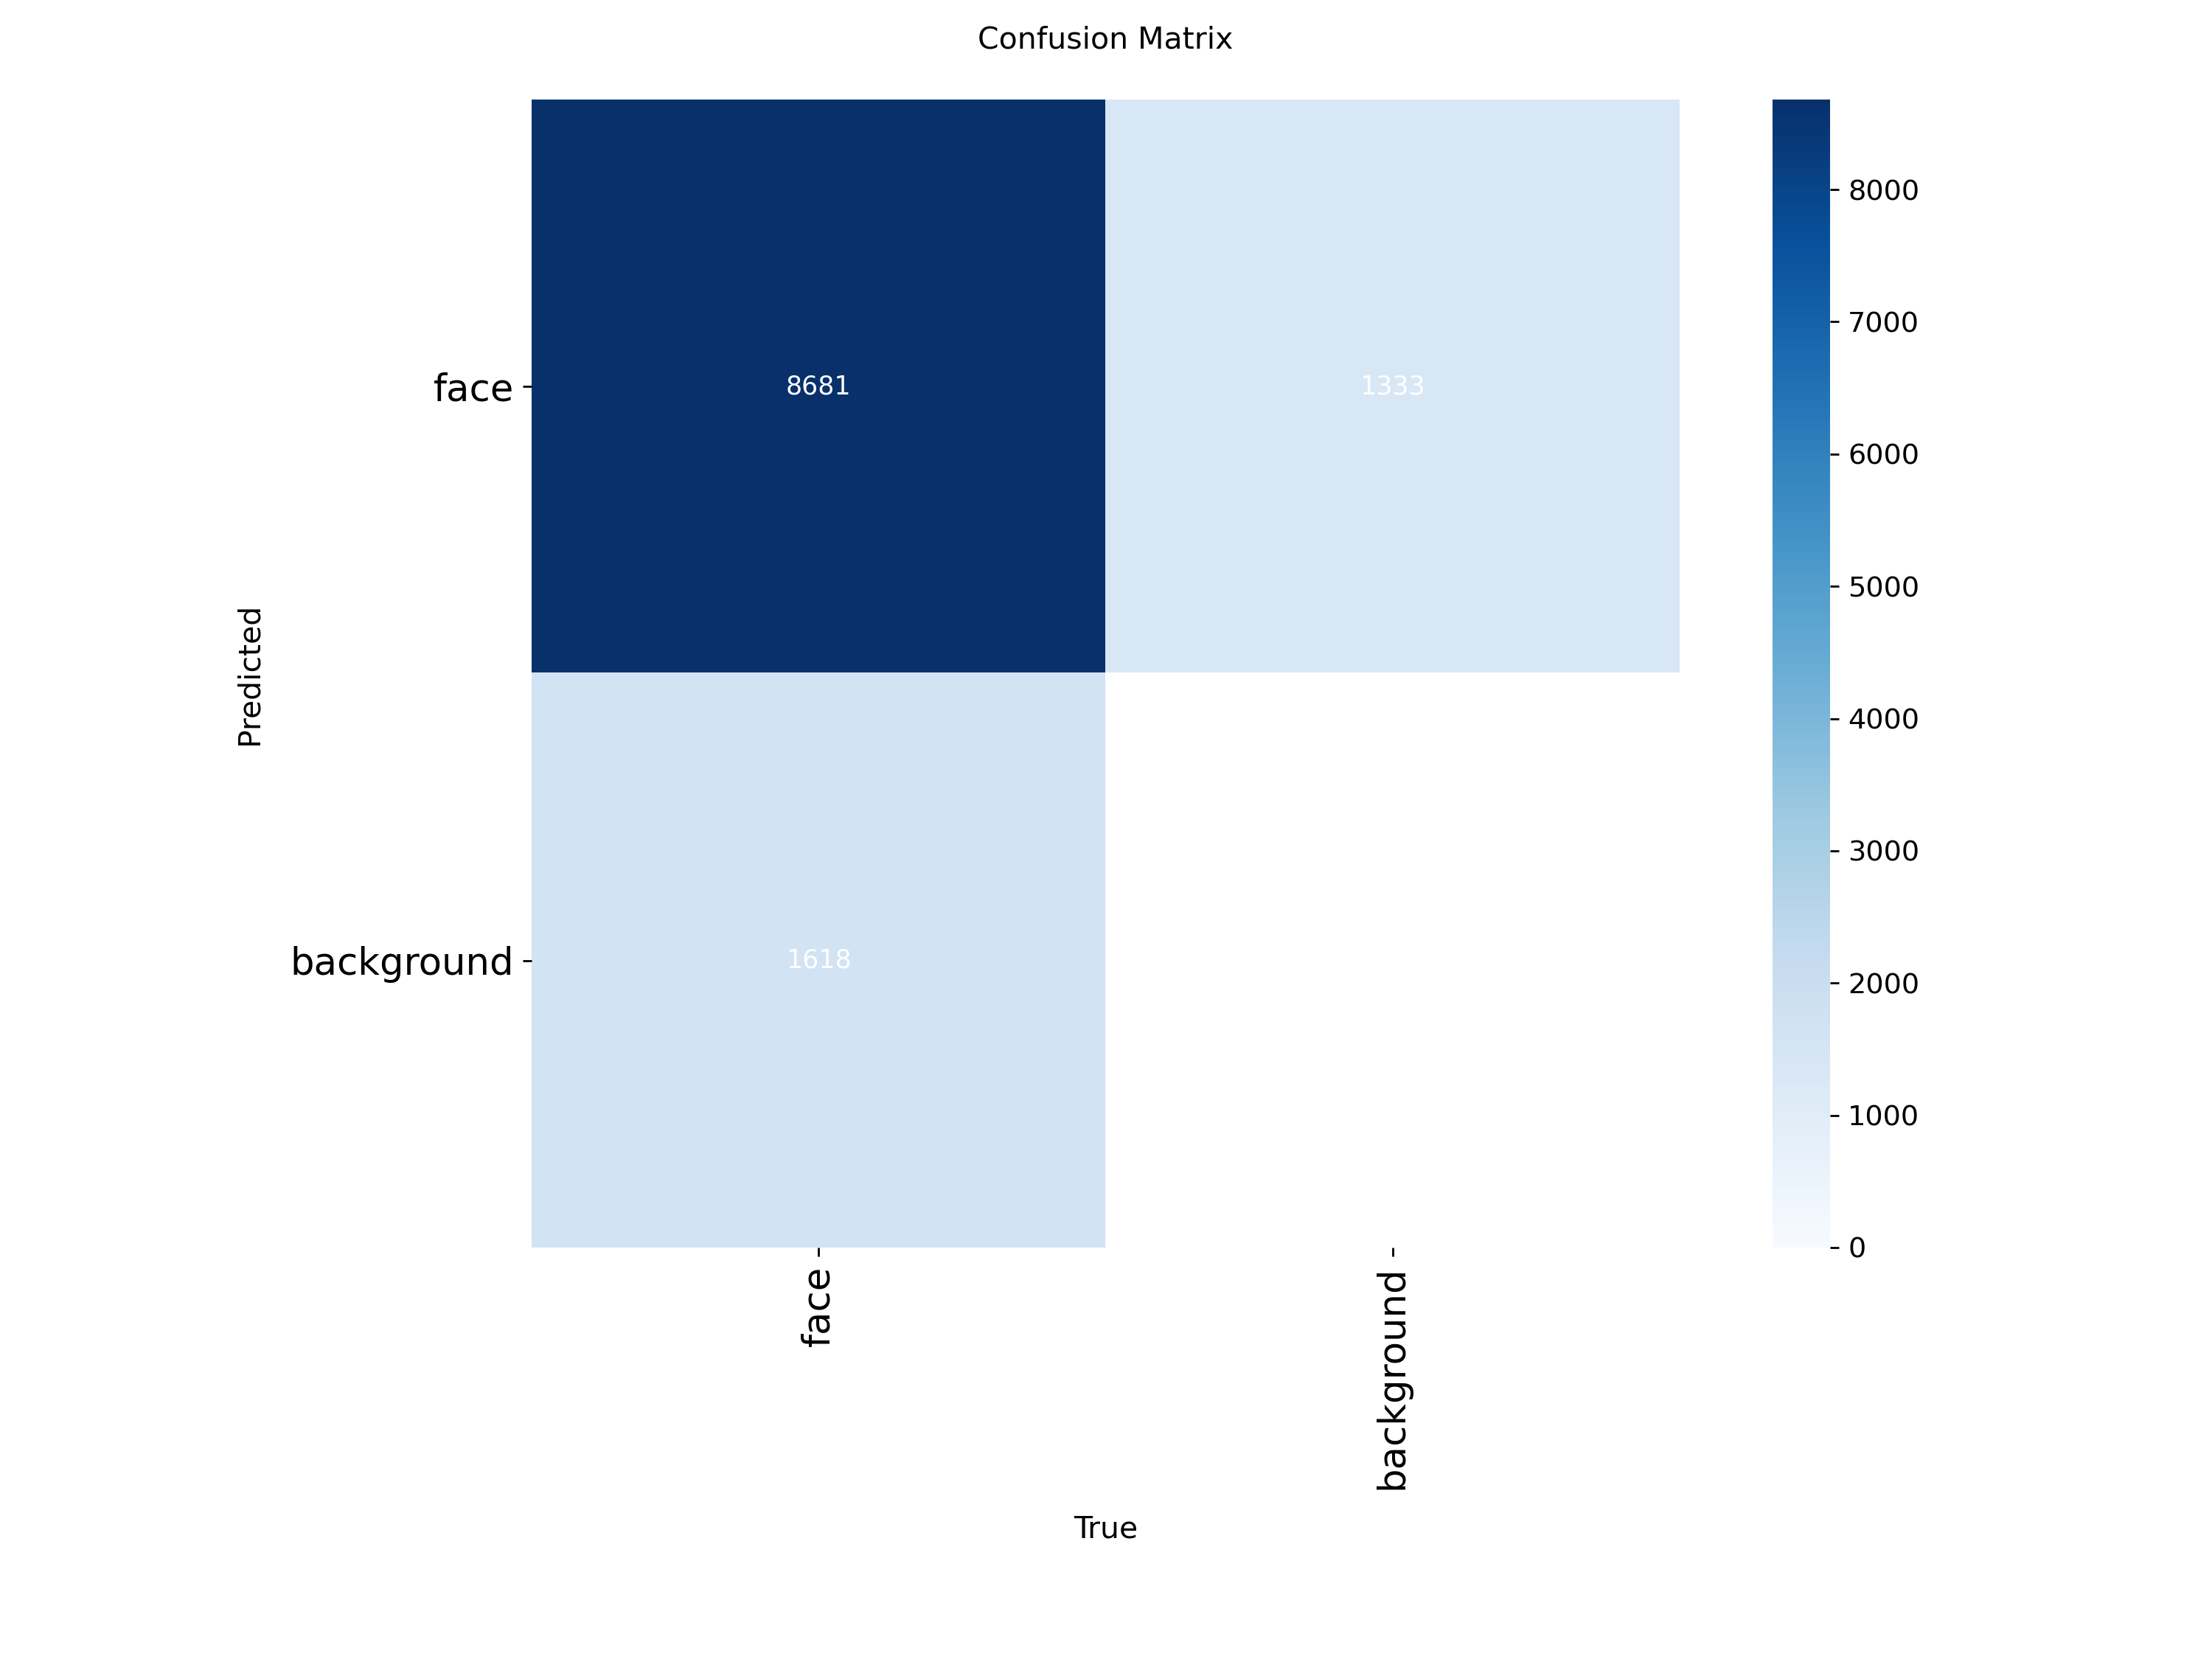
\includegraphics[width=0.6\textwidth]{figures/confusion_matrix.png}
    \caption{Konfusionsmatrix des finalen Modells auf dem Testset}
    \label{fig:confusion}
  \end{figure}
}{%
  \begin{center}
   {\color{red}\textbf{Warnung:} Bild nicht gefunden: \texttt{figures/confusion\_matrix.png}\\
  Die Konfusionsmatrix wurde in dieser Version weggelassen.}
  \end{center}
}

\section{Analyse der Ergebnisse}
Die Ergebnisse zeigen, dass das Fine-Tuning mit zu vielen freigegebenen Layern (z. B. 50) zu Overfitting führte, während ein vorsichtiger Feinschliff (10 Layer) die beste Mischung aus Precision und Recall erreichte. Die AUC-Kurve (Abbildung \ref{fig:roc}) bestätigt, dass das Modell selbst bei ungleichen Klassenverteilungen noch einigermaßen trennscharf bleibt.

\IfFileExists{figures/roc_curve.png}{%
  \begin{figure}[h]
    \centering
    \includegraphics[width=0.6\textwidth]{figures/roc_curve.png}
    \caption{ROC-Kurve (AUC = 0.7244) des finalen Modells}
    \label{fig:roc}
  \end{figure}
}{%
  \begin{center}
    {\color{red}\textbf{Warnung:} Bild nicht gefunden: \texttt{figures/roc\_curve.png}\\
    Die ROC-Kurve konnte nicht angezeigt werden.}
  \end{center}
}



% ─────────────────────────────────────────────────────────────────────────────
% 6. Diskussion
% ─────────────────────────────────────────────────────────────────────────────
%─────────────────────────────────────────────────────────────────────────────
% Kapitel 6: Diskussion
%─────────────────────────────────────────────────────────────────────────────
\chapter{Diskussion}
\label{chap:diskussion}

Obwohl das initiale Training mit eingefrorenem ResNet50 breite Generalisierung lieferte (Accuracy ~ 0,70), zeigt sich in den Feintuning-Durchläufen, dass zu umfangreiches Fine-Tuning (50 Layer) zu einer Reduktion der Recall-Rate führt (0,50 gegenüber 0,61). Mögliche Ursachen:
\begin{itemize}
  \item \textbf{Datenheterogenität:} Unterschiedliche Bildquellen (verschiedener Kaggle‐Datensätze) weisen nicht dieselben Kameraeigenschaften auf. Das Feintuning kann lokale Artefakte überanpassen.  
  \item \textbf{Overfitting:} Trotz starker L2-Regularisierung und erhöhtem Dropout (0,6) zeigten die TensorBoard‐Kurven nach Epochen 15–20 einen deutlichen Divergenz‐Effekt zwischen Training und Validierung (vgl. Anhang, Abbildung A.1).  
  \item \textbf{Fehlende große Testdaten:} Die finale Test-Stichprobe umfasste nur ca. 10 % der Bilder. Eine größere, externe Testmenge (z. B. von selbst gesammelten Realbildern) könnte die Aussagekraft verbessern.
\end{itemize}

\section{Limitationen der aktuellen Arbeit}
\begin{itemize}
  \item Systematisch wurden weder \emph{Video-Deepfakes} noch Audio-Manipulationen berücksichtigt.  
  \item Die Datensätze enthalten primär Gesichter in neutraler Mimik – extreme Gesichtsausdrücke (Lachen, Grimassen) wurden kaum repräsentiert.  
  \item Die Trainingsdauer (je Lauf 4–6 Stunden auf einer RTX 2080 Ti) begrenzte das Experimentieren mit noch tieferen Netzwerken (z. B. EfficientNetV2-Large).  
\end{itemize}


% ─────────────────────────────────────────────────────────────────────────────
% 7. Fazit
% ─────────────────────────────────────────────────────────────────────────────
%─────────────────────────────────────────────────────────────────────────────
% Kapitel 7: Fazit
%─────────────────────────────────────────────────────────────────────────────
\chapter{Fazit}
\label{chap:fazit}

Diese Projektarbeit zeigt, dass ein auf ResNet50 basierendes Transfer-Learning‐Ansatz in der Lage ist, Deepfake‐Bilder von echten Aufnahmen mit einer Accuracy von ca. 0,70 zu unterscheiden. Durch gezieltes Fine-Tuning (Freigabe nur der letzten 10 Layer) konnte ein guter Kompromiss zwischen Precision und Recall gefunden werden. Die Integration von L2‐Regularisierung und erhöhtem Dropout verhindert zumindest teilweise Overfitting. 

Für zukünftige Arbeiten wäre eine Ausweitung auf Video-Deepfakes sinnvoll, ebenso wie die Integration von multimodalen Ansätzen (z. B. Audio+Bild) und die Erforschung von Ensemble-Methoden.  

Insgesamt leistet diese Arbeit einen Beitrag zur automatisierten Erkennung von Deepfakes und kann als Grundlage für weiterführende Projekte dienen.  


% ─────────────────────────────────────────────────────────────────────────────
% Literaturverzeichnis
% ─────────────────────────────────────────────────────────────────────────────
\clearpage
\printbibliography[title={Literaturverzeichnis}]

% ─────────────────────────────────────────────────────────────────────────────
% Anhang
% ─────────────────────────────────────────────────────────────────────────────
\clearpage
%─────────────────────────────────────────────────────────────────────────────
% Anhang: Code, weitere Tabellen, TensorBoard‐Plots etc.
%─────────────────────────────────────────────────────────────────────────────
\chapter{Anhang}
\label{chap:anhang}

\section{Detailierte Versuche (Auszug)}
Im Folgenden ein Auszug aus den Versuchsdokumenten (vgl. \texttt{versuche.txt}):

\begin{itemize}
  \item ResNet50 durch EfficientNetB0 ersetzt  
  \item Functional API genutzt statt \texttt{Sequential()}  
  \item Mixed Precision aktiviert (float16)  
  \item Fehler: \enquote{Unable to serialize … JSON. Unrecognized type <EagerTensor>}  
  \item … (weitere Notizen siehe Datei \texttt{versuche.txt} im Projektordner)
\end{itemize}

\section{Zusätzliche Plots}
\begin{figure}[h]
    \centering
    \includegraphics[width=0.7\textwidth]{figures/tensorboard_training_loss.png}
    \caption{Trainingsverlauf (Loss) aus TensorBoard}
    \label{fig:tboard_loss}
\end{figure}

\section{Training‐Dokumentation (Auszug)}
Auszug aus \texttt{train_model_doku.txt} (siehe Projektordner):
\begin{quote}
“Training eines CNN-Modells zur binären Klassifikation (z.B. ‚Echt‘ vs. ‚KI-generiert‘) mit Hilfe von Transfer Learning (ResNet50) unter Verwendung von TensorFlow / Keras. …”  
\end{quote}


\end{document}
%─────────────────────────────────────────────────────────────────────────────
